\documentclass[12pt]{article}

\usepackage[utf8]{inputenc}

\usepackage[portuguese]{babel}


\usepackage{sbc-template}

\usepackage{graphicx,url}

\usepackage[brazil]{babel}   



\sloppy

\title{Relatorio EP-1}

\author{Tiago Barbosa de Lima{1}}


\address{Universidade Federal Rual de Pernambuco--PE -- Brazil
}

\begin{document} 
	
	\maketitle
	
	\begin{abstract}
		
		This report will show the collected date from the executions of some algorithms that
		use the characteristic of division and conquest comparing with the iterative algorithms and analyze their behavior using the getting graphics from the collected dates.
	\end{abstract}
	
	\begin{resumo} 
		Este relatório mostra os dados coletados a partida da execucao de alguns algoritmos do tipo de divisão e conquista comparando-os com os iterativos e analisando o seus comportamentos a parti dos gráficos obtidos a partir desses dados.
	\end{resumo}
	
	
	\section{Informações gerais}
	
	
	Os teste foram realizados usando a IDE devc++ para a elaboração dos 
	algoritmos. Alem disso todos os algoritmos foram executados a parti de um único .c.
	As chamadas de cada algoritmo foi feita a parti de  uma função que continha a versão 
	interativa e recursiva dele e por sua vez tais funções eram chamadas no "main".Foram definidas as constantes N para o valor máximo e PASSO para o tamanho a ser acrescento a entrada a cada primeira chama de cada função.
	
	
	
	
	
	\section{Algoritmo 1} \label{sec:MAX}
	
	O algoritmo MAX-REC e MAX-IT divisão e conquista e iterativo:
	
	Os algoritmos a seguir têm como objetivo devolver o 
	maior numero encontrado em um vetor de inteiros encontrado.Foram gerados valores aleatórios de inteiros baseados no tamanho da entrada.eg.: Para n igual a 2000 os valores gerados são entre 0 e 1999 e assim por diante.
	
	\begin{figure}[ht]
		\centering
		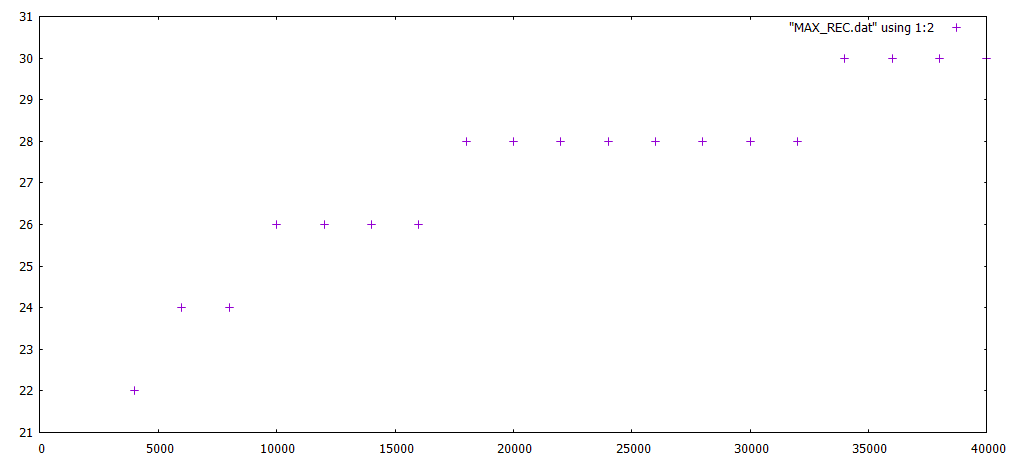
\includegraphics[width=0.7\linewidth]{Graficos/MAX_REC}
		\caption[MAX-REC]{Para realizar as 
			operações ele recebe como argumento um vetor de inteiros,
			a posição inicial e final.Ao finalizar devolve o maior valor.O gráfico de quantidade de operações realizados pela função MAX-REC em relação ao tamanho da entrada.}
		\label{fig:maxrec}
	\end{figure}
	
	
	
	\begin{figure}[ht]
		\centering
		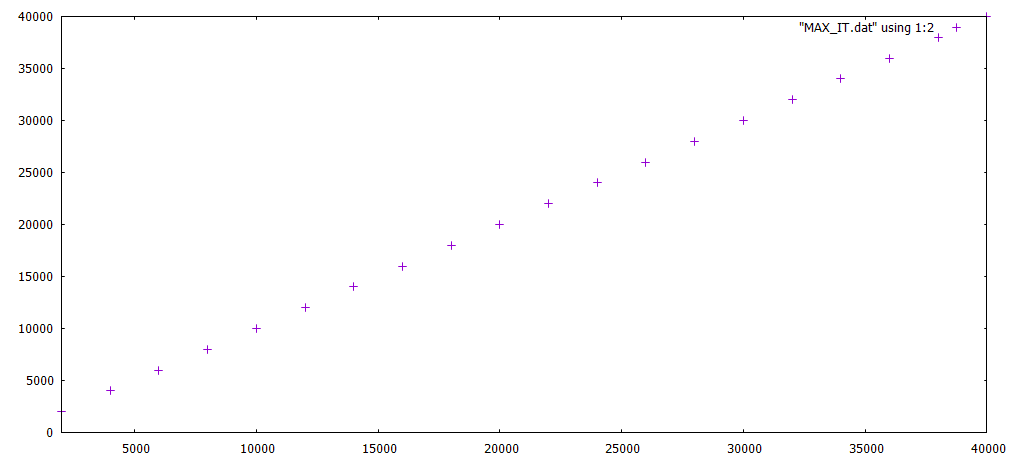
\includegraphics[width=0.7\linewidth]{Graficos/MAX_IT}
		\caption[Gráfico da função MAX-IT]{A função MAX-IT recebe como argumento um vetor de inteiros, e o seu tamanho para n maior ou igual a 0, e devolve o maior valor encontrado.Demonstra a quantidade de operações em relação ao tamanho da entrada.}
		\label{fig:maxit}
	\end{figure}
	
	\paragraph{Observações a parti dos gráficos: } Analisando o gráfico obtido a parti da execução da função MAX-REC podemos afirmar que ela tem complexidade logarítmica, ou seja ainda que para instancias de tamanhos grandes poucas operações são realizadas.Enquanto isso a função MAX-IT que realiza o mesmo procedimento de encontrar o máximo valor em vetor de inteiros, mas de maneira iterativa tem complexidade linear, ou seja, a quantidade de operações realizadas é exatamente proporcional ao tamanho da entrada como ilustra o gráfico obtido.Portanto o algoritmo recursivo mostra-se mais eficiente do que o iterativo a parti das informações obtidas a parti dos gráficos acima.
	
	\section{Algoritmo 2}\label{sec:CRESC}
	
	
	Informações preliminares: Os algoritmos a seguir têm como objetivo 
	verificar se um vetor de inteiros está em ordem crescente ou não.Os valores atribuídos ao vetor v vão de o até n-1.
	
	\subsection{Gráficos}
	\begin{figure}[h]
		\centering
		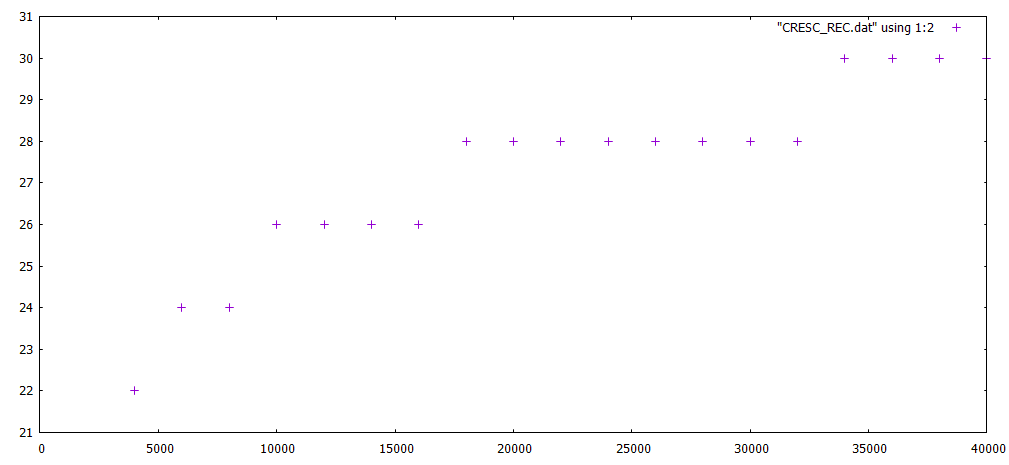
\includegraphics[width=0.7\linewidth]{Graficos/CRESC_REC}
		\caption[Gráfico CRESC-REC]{A função CRESC-REC recebe como argumento um vetor de inteiros e seu tamanho para n maior ou igual a 0, e devolve 1 se o vetor estiver ordenado e o senão devolve 1, se os valores forem iguais ele devolve a posição encontrada.O gráfico mostra a quantidade de operações em relação ao tamanho da entrada.}
		\label{fig:crescrec}
	\end{figure}
	
	\subsection{Análise}
	
	\begin{figure}[h]
		\centering
		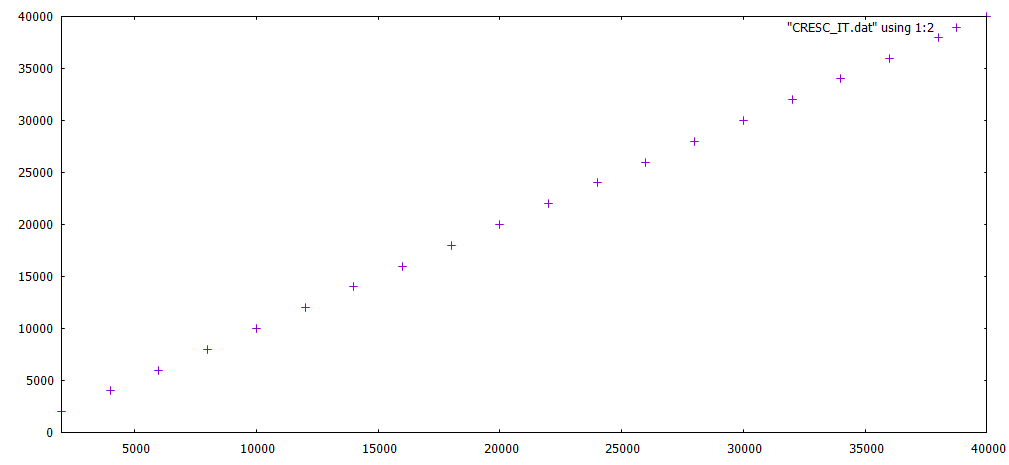
\includegraphics[width=0.7\linewidth]{Graficos/CRESC_IT}
		\caption[Gráfico CRESC-IT]{A função CRESC-IT recebe como argumento um vetor de inteiros e seu tamanho para n maior ou igual a 0 e devolve 1 se o vetor estiver ordenado e 0 senão}
		\label{fig:crescit}
	\end{figure}
	
	
	\paragraph{Observações a parti dos gráficos: }  Assim como no gráfico de MAX-REC o gráfico de CRESC-REC demonstrar ter uma complexidade logarítmica para resolução do  problema em questão enquanto o algoritmo CRESC-IT assim como MAX-IT possui uma complexidade proporcional ao tamanho da entrada n realizando portanto o mesmo ou similar quantidade de operações.Portanto o algoritmo recursivo mostra-se mais eficiente do que o iterativo a parti das informações obtidas a parti dos gráficos acima.
	
	
	
	
	
	
	
	
	\section{Algoritmo 3} \label{sec:LOC}
	
	Os algoritmos a seguir foram desenvolvidos com objetivo de localizar a posição do valor máximo em vetor de inteiros de tamanho n.
	
	
	\begin{figure}[h]
		\centering
		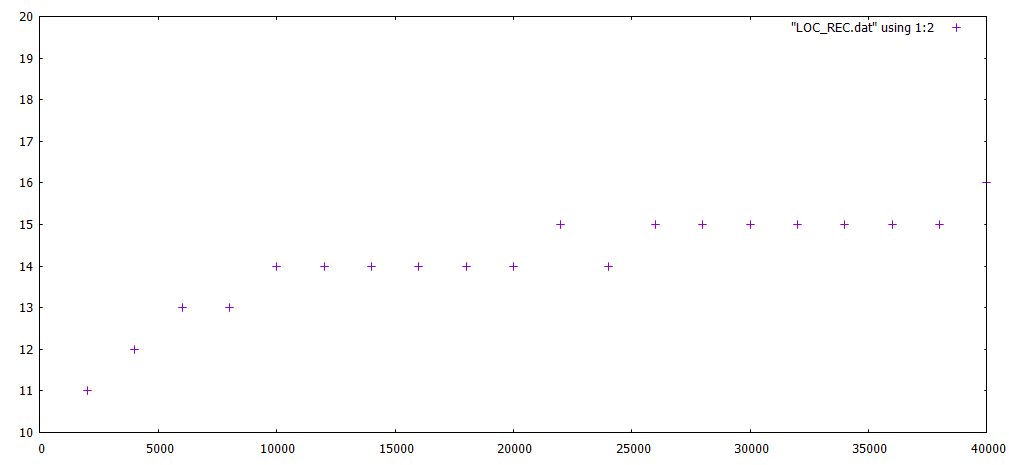
\includegraphics[width=0.7\linewidth]{Graficos/LOC_REC}
		\caption[Gráfico LOC-REC]{A função LOC-REC recebe como argumento um vetor de inteiros e o trecho e inicial e final do trecho analisado, e devolve a posição do valor x encontrado ou o que mais se aproxima baseado no LOC-IT feito em sala.}
		\label{fig:locrec}
	\end{figure}
	
	\begin{figure}[h]
		\centering
		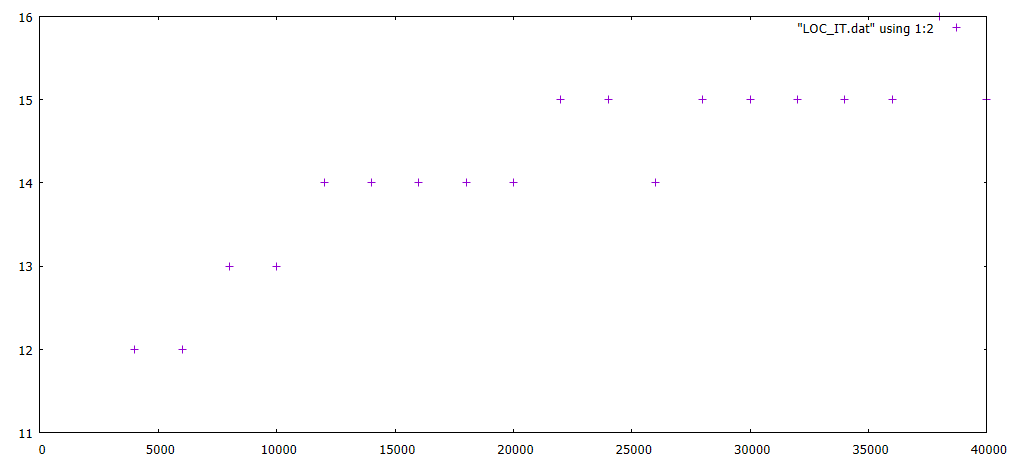
\includegraphics[width=0.7\linewidth]{Graficos/LOC_IT}
		\caption[Gráfico LOC-IT]{A função LOC-IT recebe como argumento um vetor de inteiros o seu tamanho o valor e o x a serem encontrado e devolve a sua posição ou a posição relativa ao valor mais próximo.Obs.: Algoritmo feito na sala de aula.}
		\label{fig:locit}
	\end{figure}
	
	
	\paragraph{Observações a parti dos gráficos: } Diferentemente dos algoritmos anteriores em que o algoritmo recursivo se mostrava ter uma complexidade melhor do que a do iterativo, podemos observar que a depender da posição do valor a ser encontrado ambos algoritmos (recursivo e iterativo) têm a mesma complexidade.Portanto ambos os dois mostram-se eficientes a parti das informações obtidas a parti dos gráficos acima.
	
	\section{Algoritmo 4} \label{sec: SEG}
	Os algoritmos a seguir têm como objetivo encontrar o valor da soma máxima dentro de um vetor de inteiros e devolver esse valor.No caso do vetor ser formado por apenas números negativos o valor devolvido será o valor menos negativo.
	
	
	\begin{figure}[ht]
		\centering
		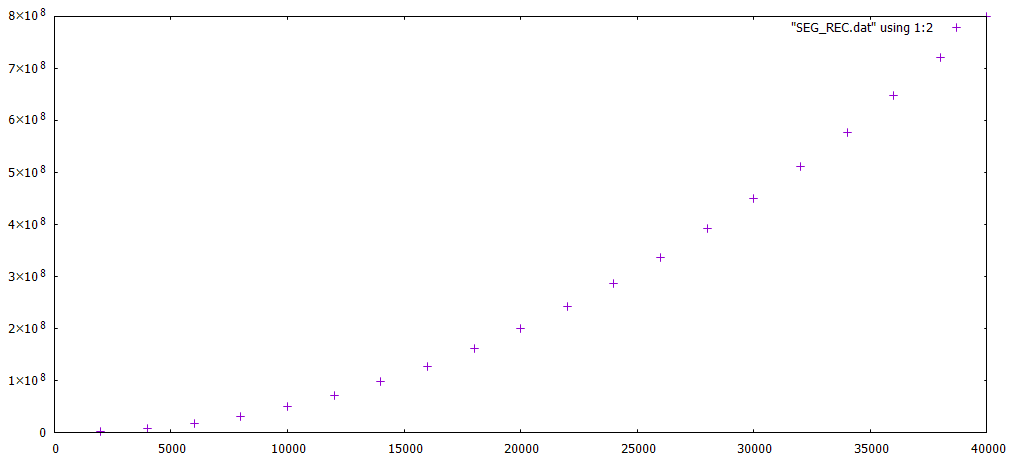
\includegraphics[width=0.7\linewidth]{Graficos/SEG_REC}
		\caption[Gráfico SEG-REC]{A função SEG-REC recebe como argumento um vetor de inteiros e seu tamanho para n maior ou igual a 0, além da valor inicial da soma que deve ser 0 e devolve o maior seguimento de soma do vetor de entrada. Fonte: https://www.ime.usp.br/~pf/livrinho-AA/AA-BOOKLET.pdf}
		\label{fig:segrec}
	\end{figure}
	
	\pagebreak
	\begin{figure}[t]
		\centering
		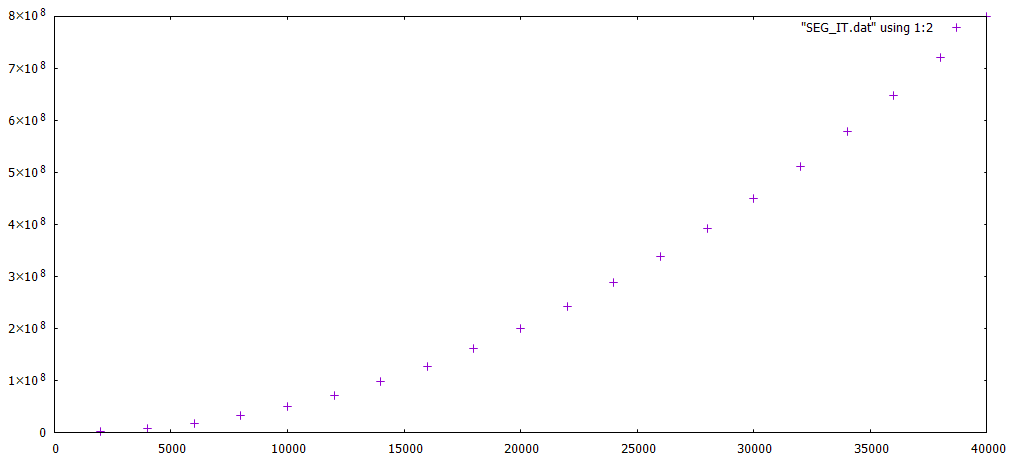
\includegraphics[width=0.7\linewidth]{Graficos/SEG_IT}
		\caption[Gráfico SEG-IT]{A função SEG-IT recebe como argumento um vetor de inteiros e seu tamanho para n maior ou igual a 0 e devolve a soma do vetor v máxima FONTE: https://www.ime.usp.br/~pf/livrinho-AA/AA-BOOKLET.pdf}
		\label{fig:segit}
	\end{figure}
	
	
	\paragraph{Observações a parti dos gráficos: } 
	Neste gráficos podemos observar que o algoritmo iterativo apresenta uma complexidade exponencial tendo que realizar uma quantidade enorme de operações. Enquanto o algoritmo recursivo a presenta uma complexidade logarítmica realizando um quantidade menor de operações apesar da entrada ser grande.
	
	
	
	
	\bibliographystyle{sbc}
	\bibliography{sbc-template}
	https://www.ime.usp.br/~pf/livrinho-AA/AA-BOOKLET.pdf
	
	https://pt.khanacademy.org/computing/computer-science/algorithms/merge-sort/a/divide-and-conquer-algorithms
	
	
\end{document}

